Suppose we are parsing a sentence ``submit the homework through Canvas" with a Probability Context Free Grammar (PCFG) in Chomsky Normal Form. We give the PCFG as follows.

\begin{table}[h]
\centering
\begin{tabular}{|l|l|}
\hline
Rule & Probability  \\ \hline
S $\longrightarrow$ NP VP &  0.8       \\ \hline
S $\longrightarrow$ submit &    0.01      \\ \hline
S $\longrightarrow$ Verb NP &    0.05     \\ \hline
S $\longrightarrow$ VP PP &    0.03     \\ \hline
NP $\longrightarrow$ Canvas &    0.16     \\ \hline
NP $\longrightarrow$ Gradescope &    0.04     \\ \hline
NP $\longrightarrow$ Det Nominal &    0.6     \\ \hline
Nominal $\longrightarrow$ Nominal Noun &    0.2     \\ \hline
Nominal $\longrightarrow$ Nominal PP &    0.5     \\ \hline
Nominal $\longrightarrow$ homework &    0.15     \\ \hline
VP $\longrightarrow$ submit &    0.1     \\ \hline
VP $\longrightarrow$ contain &    0.04     \\ \hline
VP $\longrightarrow$ Verb NP &    0.5    \\ \hline
VP $\longrightarrow$ VP PP &    0.3    \\ \hline
PP $\longrightarrow$ Prep NP &    1.0    \\ \hline
Det $\longrightarrow$ the &    0.6    \\ \hline
Prep $\longrightarrow$ through &    0.2    \\ \hline
Verb $\longrightarrow$ submit &    0.5    \\ \hline


\end{tabular}\caption{Initial probabilities} \label{Tab:Initial}
\end{table}



\begin{enumerate}
    \item Parse the sentence  ``submit the homework through Canvas'' by using the CKY Algorithm. You need to show the probabilities of all possible parses and choose the parse with the highest probability. Please show all the steps of calculations. [8 pts]
    
    \item Compute the probability of the given sentence ``submit the homework through Canvas'' by using the CKY Algorithm. Please show all the steps of calculations.  [2 pts]
    

\end{enumerate}

\begin{solution}
a)

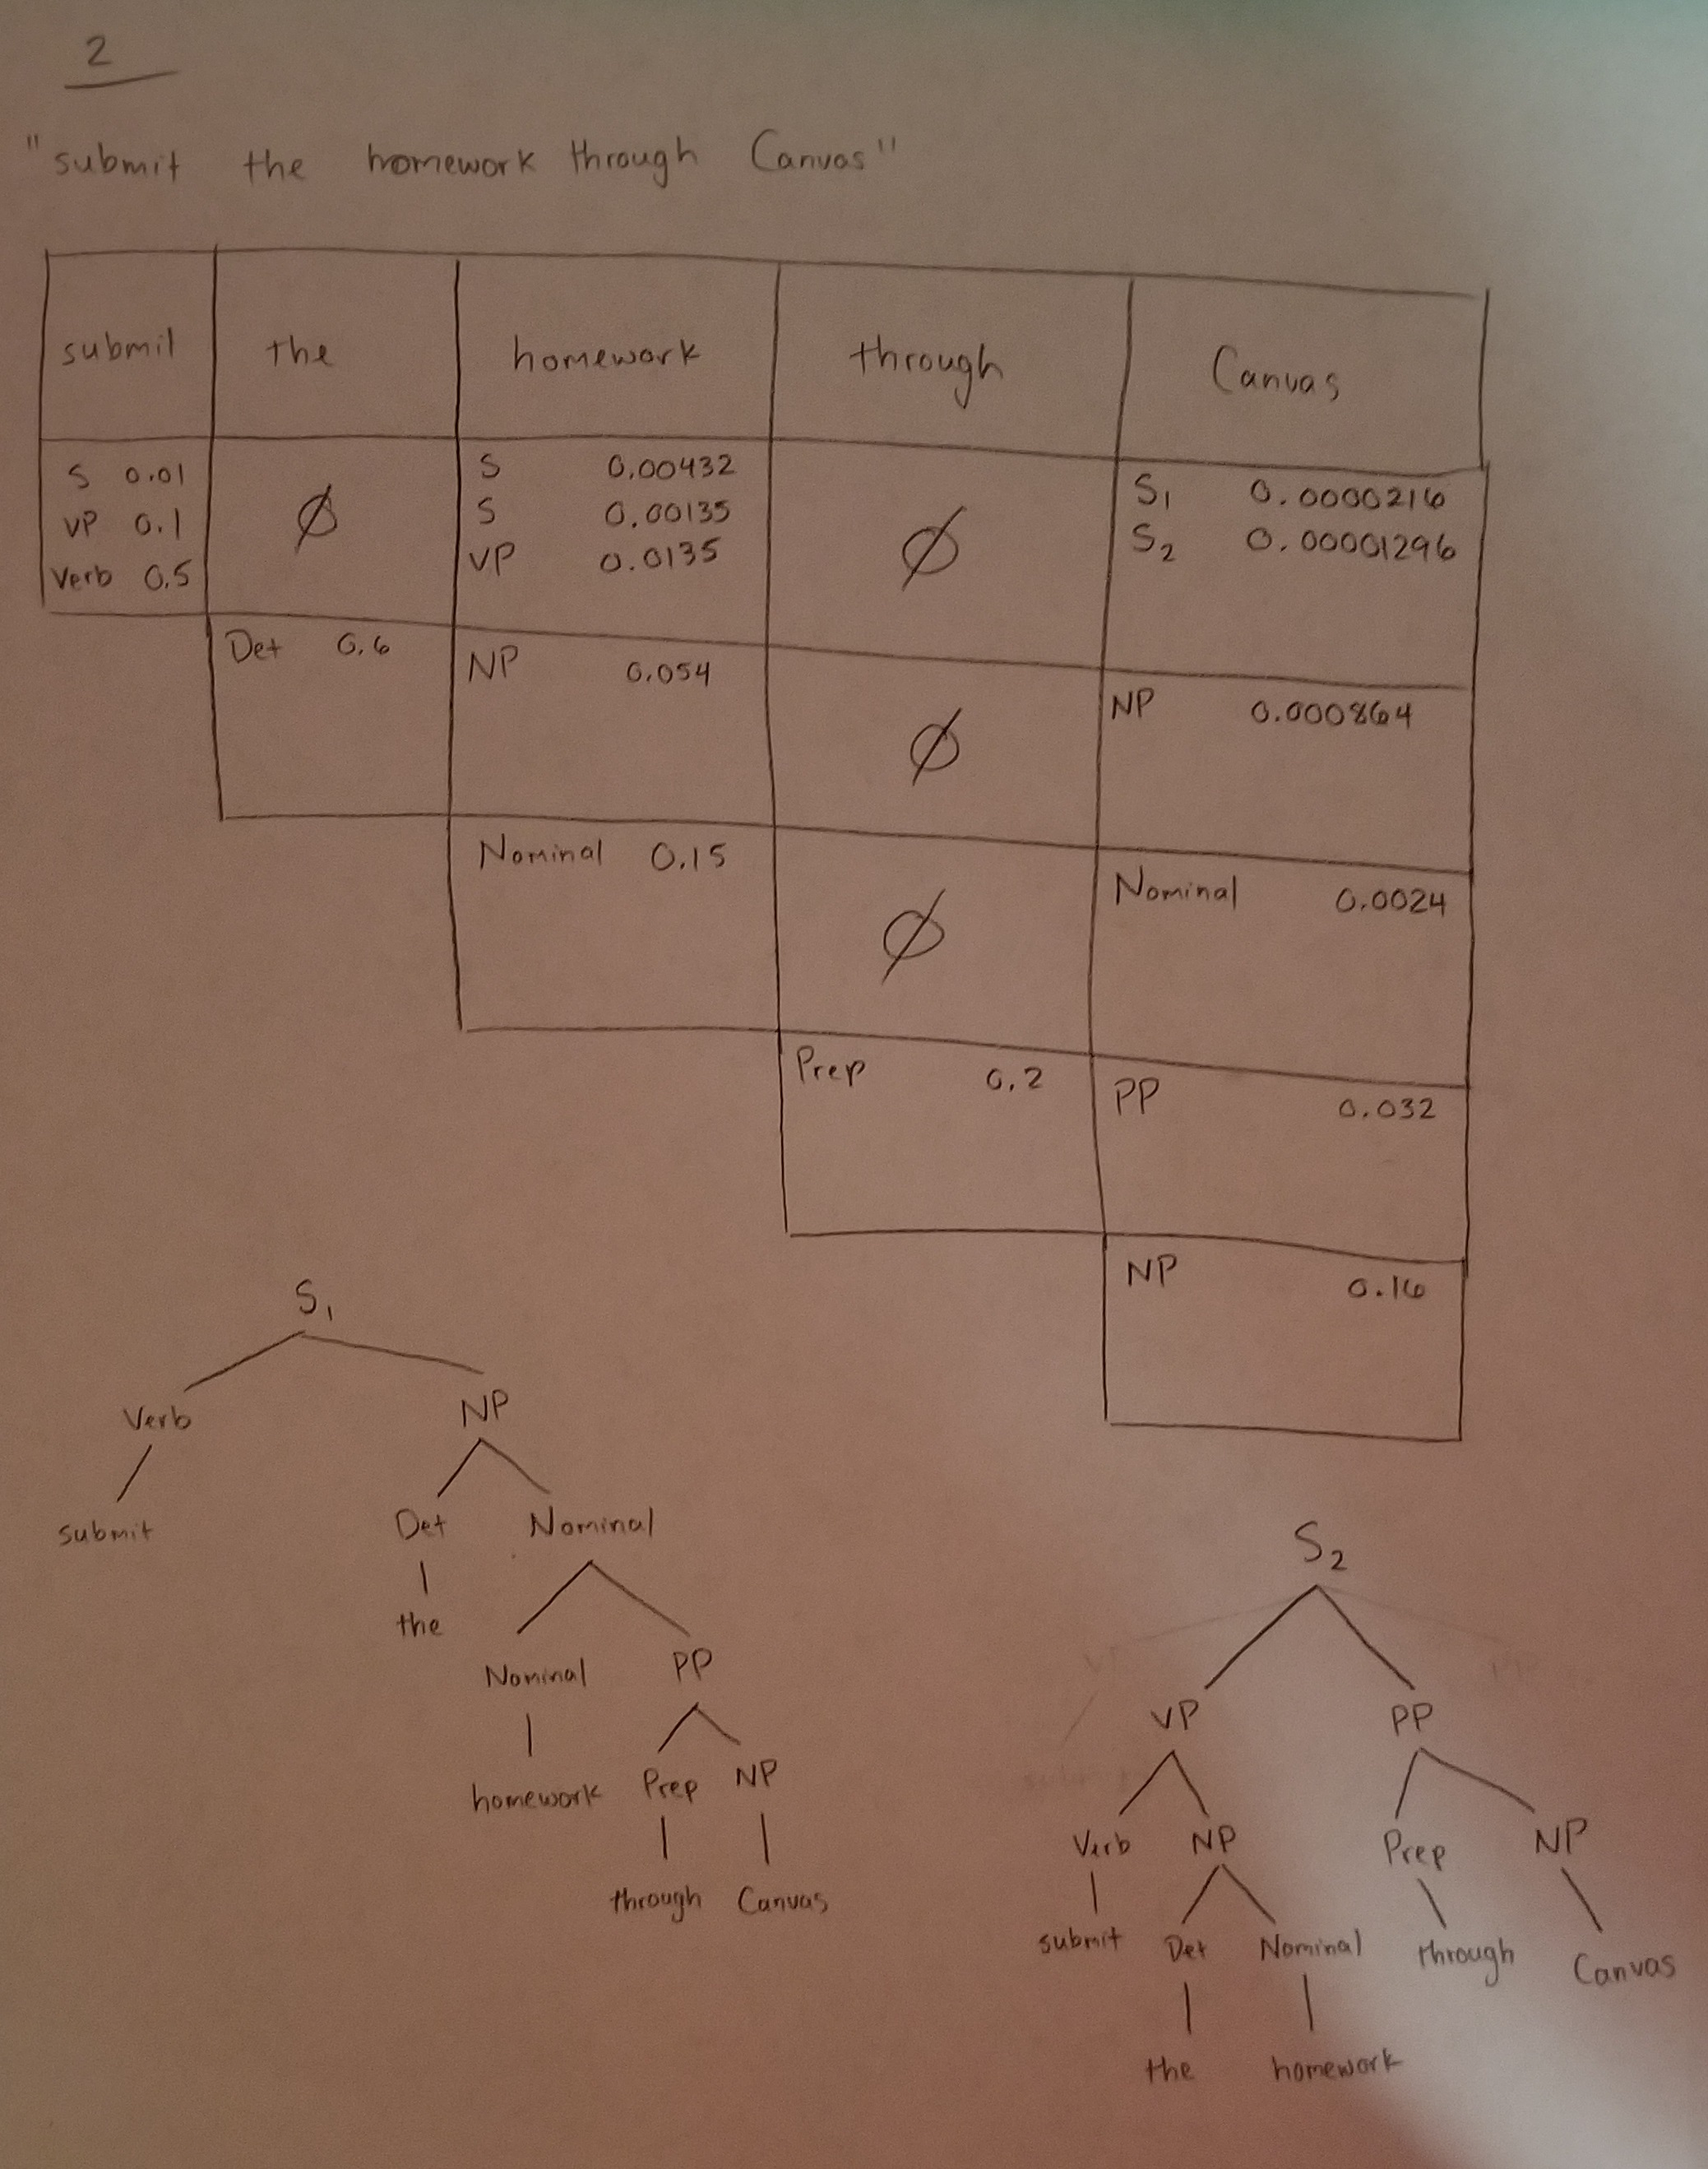
\includegraphics[scale=0.15]{q2-a}

From the above picture, one can see 2 parses were found, $S_1$ and $S_2$. The probability of each parse is as follows: $P(S_1) = 0.0000216$, $P(S_2) = 0.00001296$. The parse with the highest probability is $S_1$, and its parse tree is shown in the above picture, with the following chronological tags: Verb Det Nominal Prep NP.

b)

$P(S_1) = 0.0000216\\
P(S_2) = 0.00001296$

So, $P(S) = P(S_1) + P(S_2) = \mathbf{0.00003456}$
\end{solution}